\documentclass[aspectratio=169,11pt]{beamer}
\usetheme{Madrid}
\usecolortheme{default}
\usepackage[utf8]{inputenc}
\usepackage[T2A]{fontenc}
\usepackage[russian]{babel}
\usepackage{amsmath}
\usepackage{booktabs}
\usepackage{tabularx}
\usepackage{array}
\usepackage{graphicx}
\usepackage{hyperref}
\usepackage{multimedia}

\graphicspath{{presentation_assets/}}

\title{Финансовый помощник по инструментам Московской Биржи на основе RAG}
\subtitle{Магистерский проект}
\author{Охотин Даниил \and Ващин Леонид \and Гусев Владислав}
\institute{НИУ ВШЭ}
\date{2026}

\begin{document}

\begin{frame}
  \titlepage
\end{frame}

\begin{frame}{Постановка задачи}
  \small
  \textbf{Предметная область.} Пользователь задает вопросы о финансовых инструментах, налоговых режимах, биржевой инфраструктуре и инвестиционных продуктах. Источники ответа должны быть контролируемыми и воспроизводимыми, а не целиком зависеть от памяти LLM.

  \vspace{0.4em}
  \textbf{Цель проекта.} Реализовать RAG-сервис, который:
  \begin{itemize}
    \item извлекает релевантные документы из локального корпуса;
    \item ранжирует кандидатов так, чтобы в контекст генератора попадали именно полезные фрагменты;
    \item формирует финальный ответ на основе найденного контекста;
    \item собирает пользовательский feedback и превращает его в данные для дообучения retrieval-части.
  \end{itemize}

  \vspace{0.4em}
  \textbf{Практическая польза.}
  \begin{itemize}
    \item Для клиентов брокера: быстрое объяснение терминов и процедур без ручного поиска по базе знаний.
    \item Для поддержки: единообразные ответы на повторяющиеся вопросы.
    \item Для продуктовой команды: логи запросов, метрики качества, сигналы для пополнения и улучшения корпуса.
  \end{itemize}
\end{frame}

\begin{frame}{Описание данных}
  \small
  \begin{columns}[T]
    \begin{column}{0.56\textwidth}
      \begin{itemize}
        \item \textbf{Основной корпус:} 4\,795 чанков статей T-Bank и 7\,008 чанков теоретических материалов в финальном формате папки \texttt{data/}.
        \item \textbf{Структура записи:} \texttt{chunk\_id}, \texttt{text}, \texttt{meta}; исходные ML-скрипты были адаптированы под chunk-level JSON вместо article-level схемы.
        \item \textbf{Поля meta:} \texttt{character\_count}, \texttt{original\_character\_count}, \texttt{source\_file}, \texttt{translated\_from\_english}.
        \item \textbf{Golden set:} 670 исходных вопросов; после фильтрации и сопоставления с корпусом для offline retrieval используется 627 QA-пар. Для быстрых MLflow-прогонов в репозитории зафиксирована выборка из 20 запросов.
      \end{itemize}
    \end{column}
    \begin{column}{0.44\textwidth}
      \footnotesize
      \begin{tabular}{lrr}
        \toprule
        Корпус & T-Bank & Theory \\
        \midrule
        Чанков & 4\,795 & 7\,008 \\
        Медиана, симв. & 839 & 1\,031 \\
        Среднее, симв. & 946 & 1\,027 \\
        P95, симв. & 2\,180 & 1\,157 \\
        Пропуски текста & 0 & 0 \\
        \bottomrule
      \end{tabular}
    \end{column}
  \end{columns}
\end{frame}

\begin{frame}{EDA: длины и форма распределений}
  \small
  \begin{columns}[T]
    \begin{column}{0.58\textwidth}
      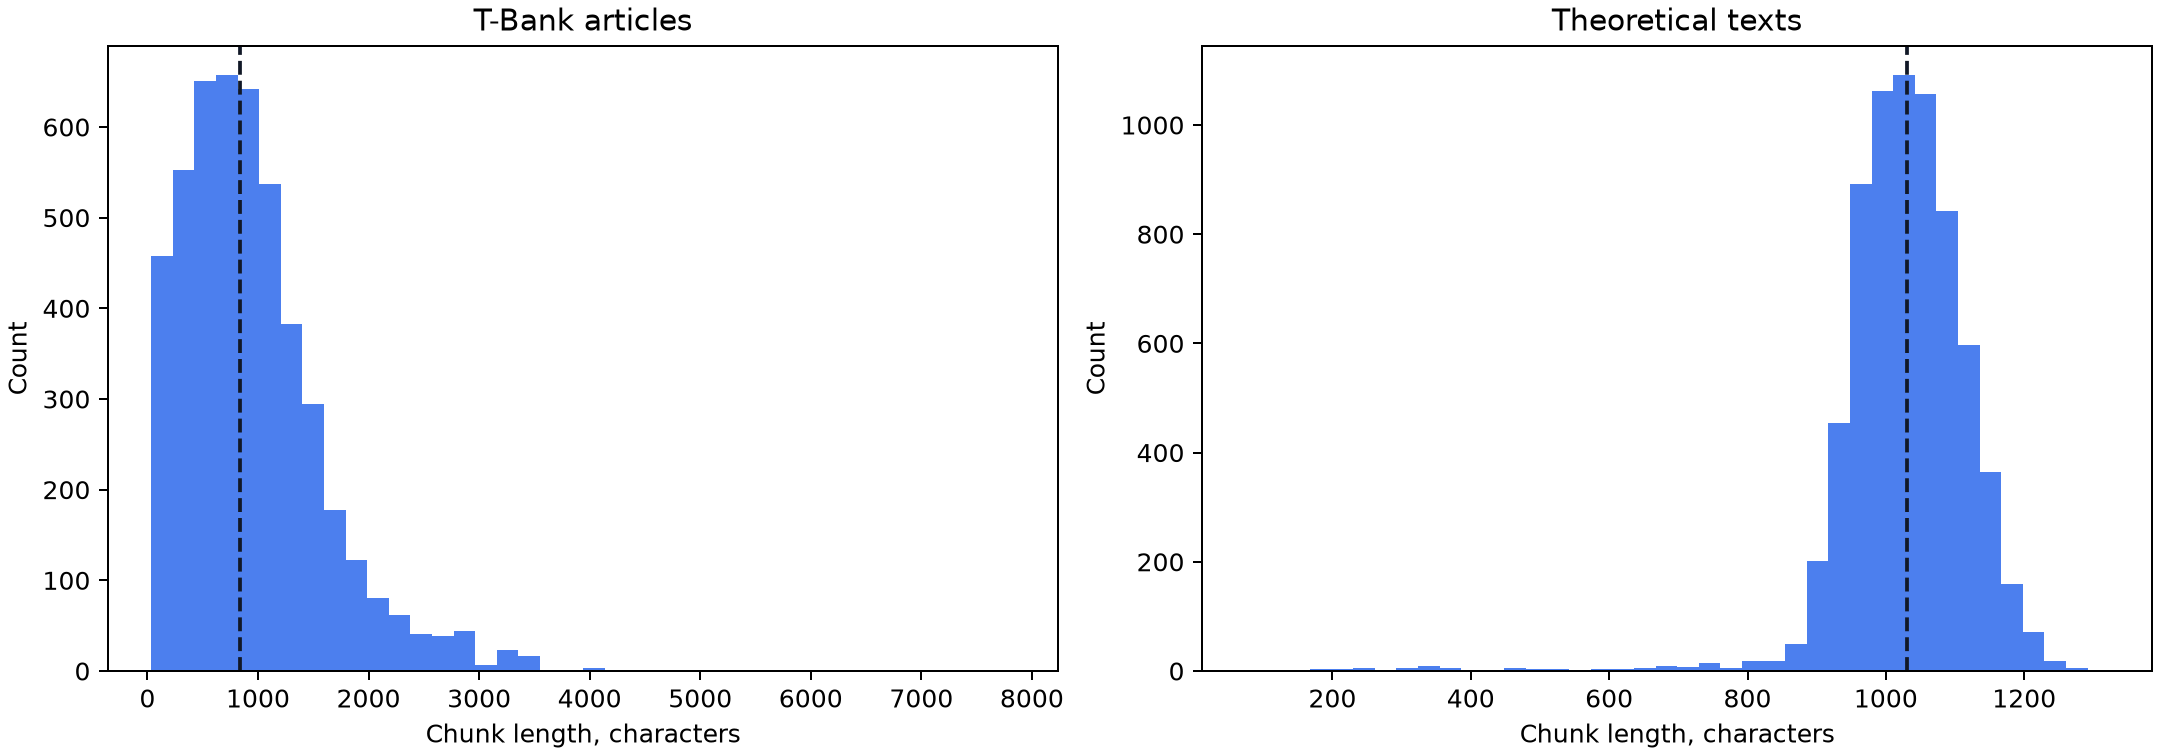
\includegraphics[width=\textwidth]{eda_text_lengths.png}
    \end{column}
    \begin{column}{0.42\textwidth}
      \footnotesize
      \begin{itemize}
        \item Корпус T-Bank заметно более разреженный по длине: есть и короткие служебные фрагменты, и длинные хвостовые чанки после склейки абзацев.
        \item Теоретические тексты существенно стабильнее по размеру: большинство чанков лежит около 1\,000 символов и ближе к регулярному режиму нарезки.
        \item Для retrieval это важно: слишком короткие фрагменты хуже сохраняют определение термина, а слишком длинные усложняют reranking, замедляют cross-encoder и повышают риск шумного контекста в генерации.
        \item Длинный хвост у T-Bank объясняет, почему полнодокументное представление и крупные чанки показывают более сильный Recall@5, чем агрессивный мелкий chunking.
      \end{itemize}
    \end{column}
  \end{columns}
\end{frame}

\begin{frame}{EDA: качество корпуса и golden set}
  \small
  \begin{columns}[T]
    \begin{column}{0.5\textwidth}
      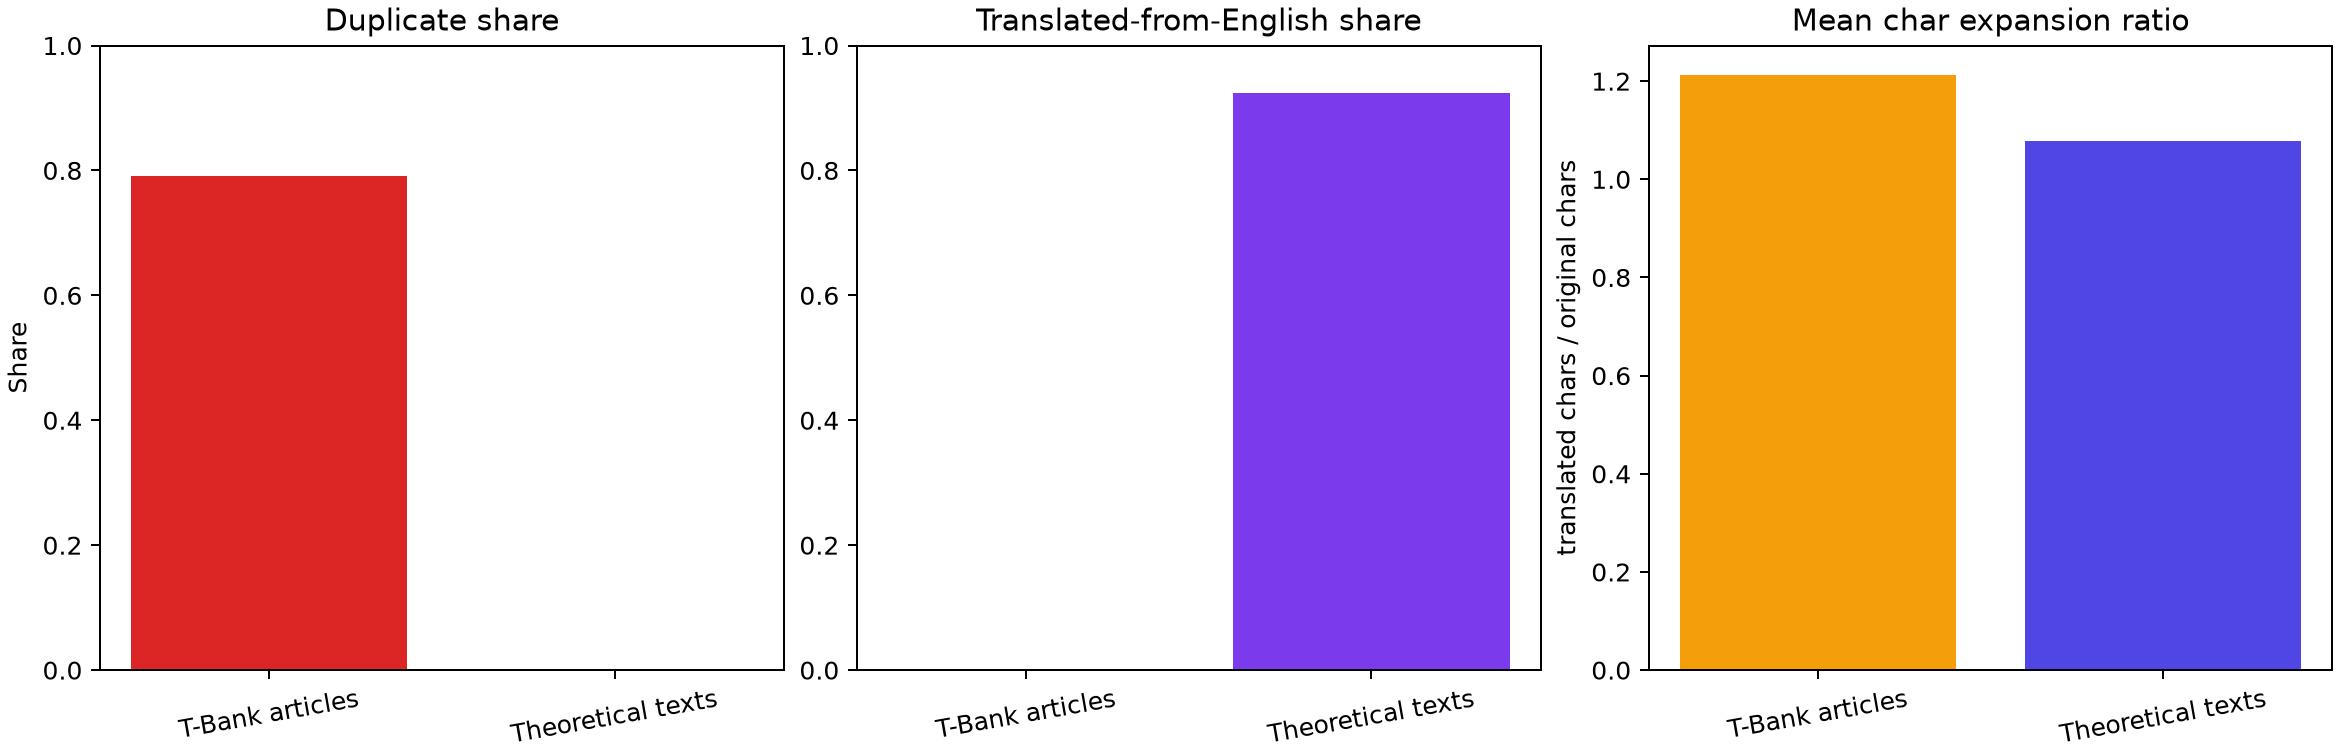
\includegraphics[width=\textwidth]{eda_dataset_quality.png}
    \end{column}
    \begin{column}{0.5\textwidth}
      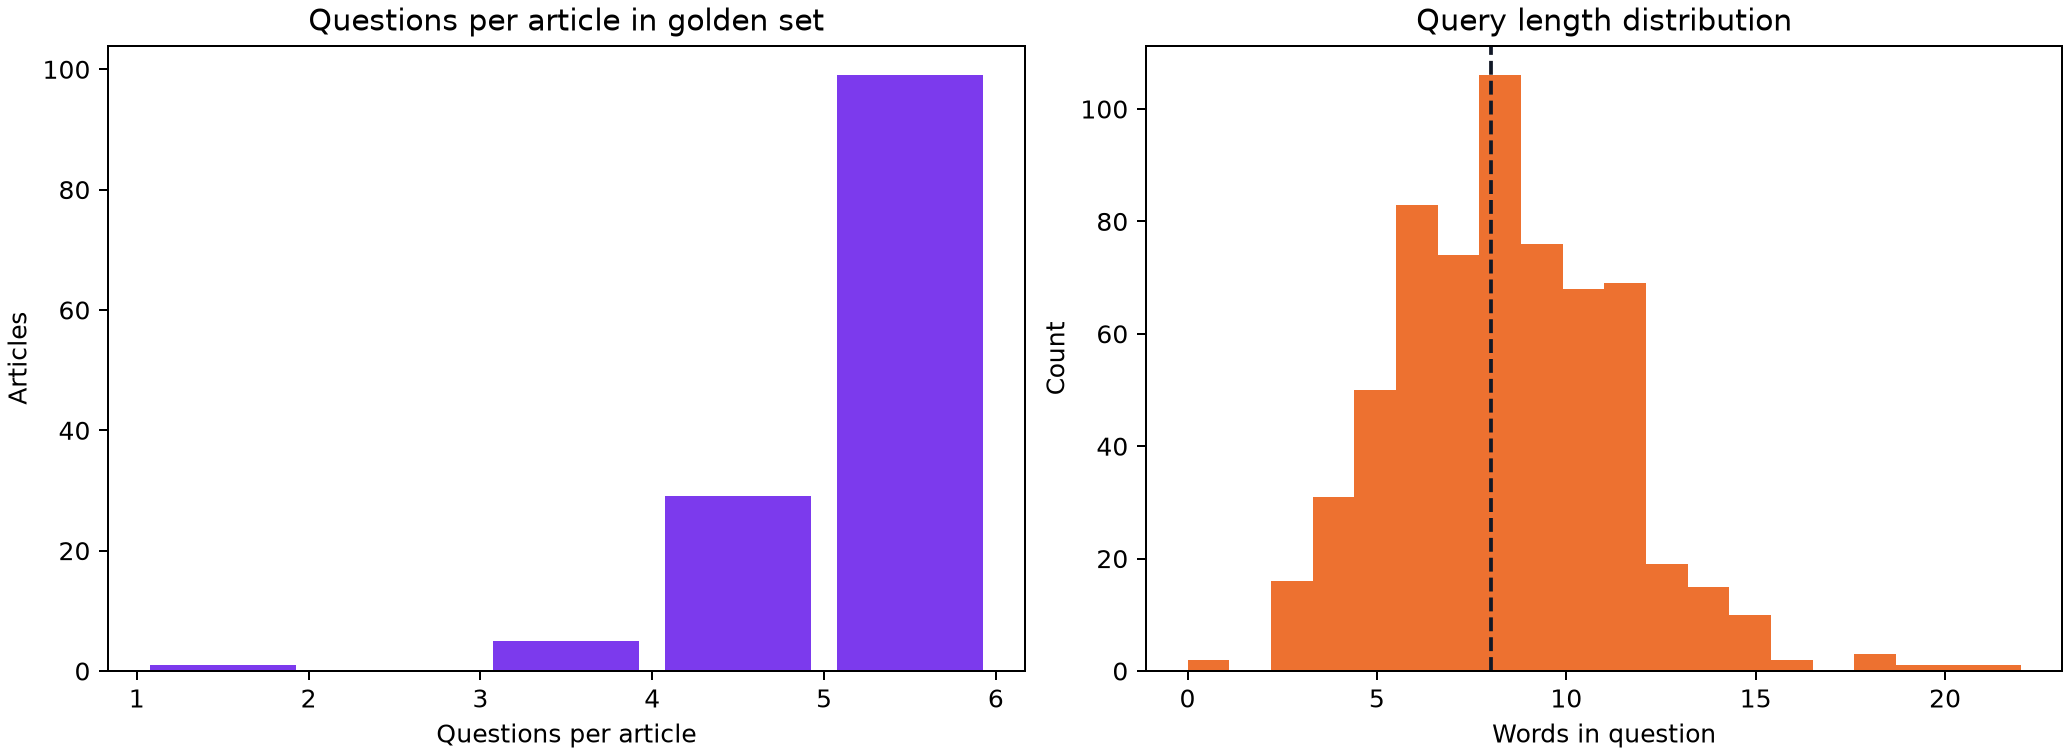
\includegraphics[width=\textwidth]{eda_golden_set.png}
    \end{column}
  \end{columns}
  \vspace{0.3em}
  \footnotesize
  \begin{itemize}
    \item В T-Bank доля дубликатов очень высока: около 79\%, поэтому при оценке важно не путать близкие повторяющиеся чанки с настоящим улучшением retrieval и не завышать качество за счет near-duplicate выдачи.
    \item В теоретическом корпусе преобладают переведенные источники; среднее расширение текста после перевода около 1.08x, что влияет на длину чанков, плотность терминов и стиль формулировок.
    \item Golden set в основном содержит 4--5 вопросов на статью, а длины запросов умеренны; это ближе к реальным пользовательским сценариям, чем длинные академические формулировки.
  \end{itemize}
\end{frame}

\begin{frame}{EDA: состав теоретического корпуса и выводы}
  \small
  \begin{columns}[T]
    \begin{column}{0.55\textwidth}
      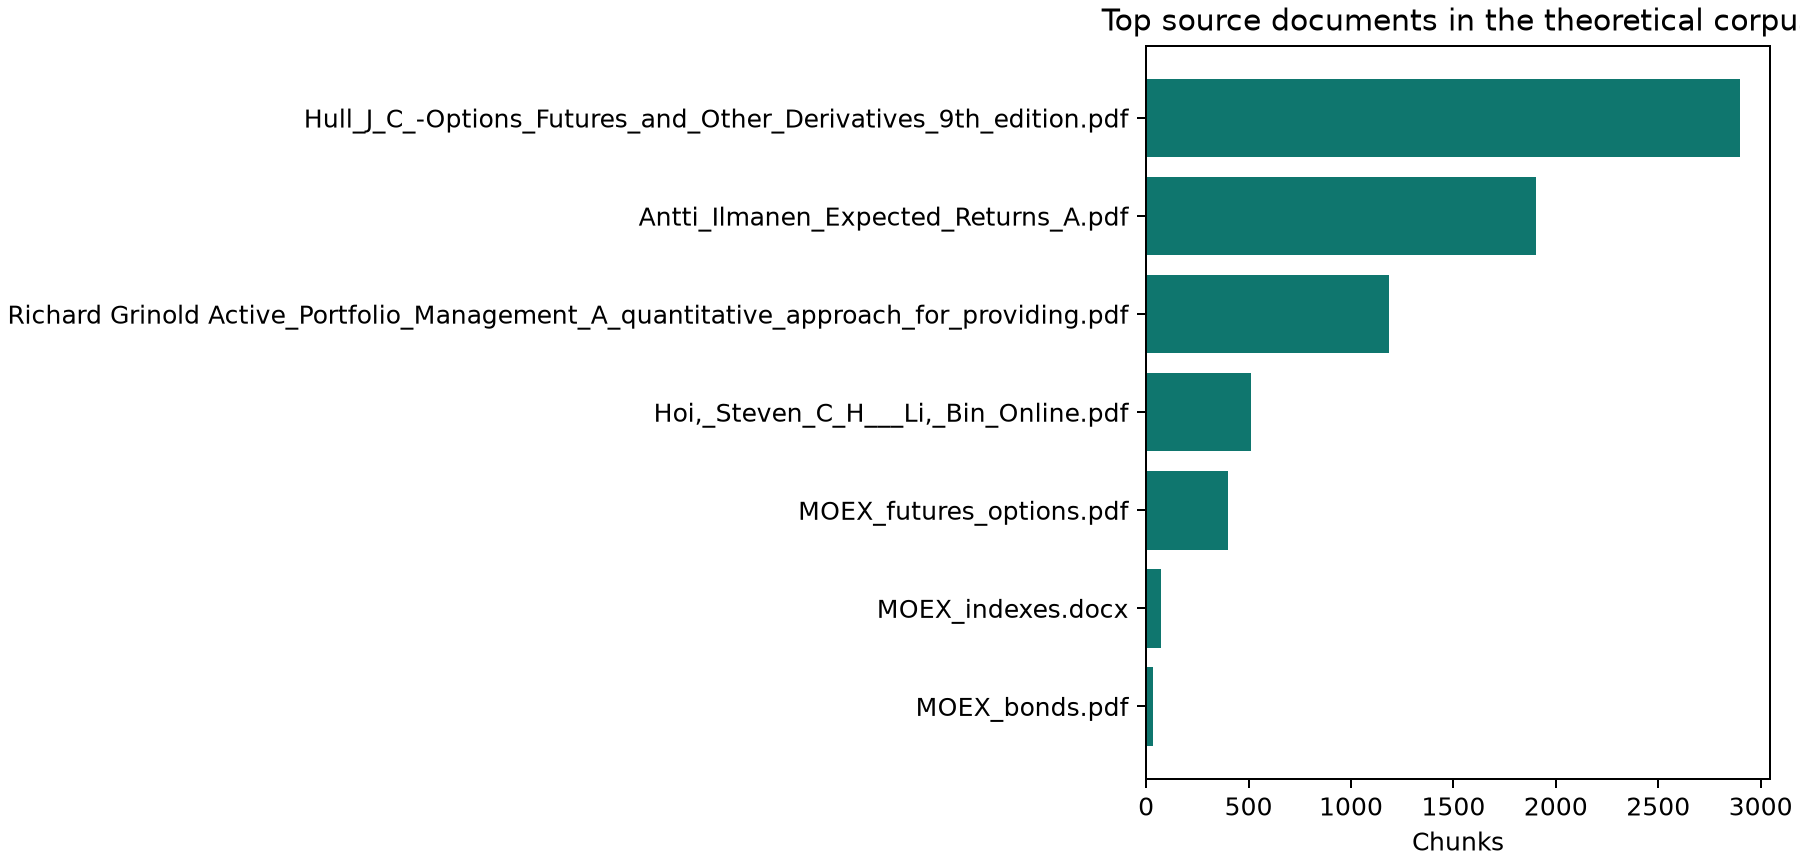
\includegraphics[width=\textwidth]{eda_theoretical_sources.png}
    \end{column}
    \begin{column}{0.45\textwidth}
      \footnotesize
      \textbf{Наблюдения:}
      \begin{itemize}
        \item Наибольший вклад дают несколько крупных источников: Hull, Ilmanen, Grinold.
        \item Корпус смещен в сторону англоязычной академической литературы и переводных материалов, поэтому терминология богаче, но стиль и уровень детализации отличаются от клиентских FAQ-статей.
      \end{itemize}

      \vspace{0.3em}
      \textbf{Выводы для решения:}
      \begin{itemize}
        \item Главной метрикой retrieval лучше делать Recall@K: для RAG-контекста критично, чтобы корректный источник вообще попал в top-$K$.
        \item Precision@K интерпретируется как «чистота» контекста, а не как абсолютная полнота: LLM работает лучше, когда среди top-$K$ меньше тематического шума.
        \item Для production-сценария нужен отдельный rerank, потому что один dense retrieval плохо различает близкие финансовые термины, синонимичные объяснения и повторяющиеся чанки.
      \end{itemize}
    \end{column}
  \end{columns}
\end{frame}

\begin{frame}{Метрики: формулы и интерпретация}
  \small
  Для запроса $q$ пусть $Rel(q)$ --- множество релевантных документов, а $TopK(q)$ --- первые $K$ результатов retrieval.

  \vspace{0.2em}
  \[
    Precision@K(q) = \frac{|TopK(q) \cap Rel(q)|}{K}
  \]
  \[
    Recall@K(q) = \frac{|TopK(q) \cap Rel(q)|}{|Rel(q)|}
  \]
  \[
    MRR = \frac{1}{|Q|} \sum_{q \in Q} \frac{1}{rank_q}
  \]

  \footnotesize
  \begin{itemize}
    \item В нашем golden set на запрос обычно приходится один основной релевантный документ, поэтому Recall@5 эквивалентен вероятности попадания правильного источника в контекст.
    \item Precision@1 важен как proxy пользовательского доверия: если верхний документ нерелевантен, даже хороший Recall@5 не гарантирует качественный ответ.
    \item MRR показывает, насколько высоко расположен первый релевантный документ и помогает сравнивать ранжирование при близких Recall@K.
  \end{itemize}
\end{frame}

\begin{frame}{Базовое решение}
  \small
  \begin{itemize}
    \item Стартовый baseline: BM25 + bi-encoder + простая подача найденного контекста в LLM.
    \item Для dense retrieval использовался \texttt{sentence-transformers/paraphrase-multilingual-MiniLM-L12-v2}; корпус при этом предварительно восстанавливался из chunk-level формата в article/document-level представление.
    \item На document-level retrieval baseline дал $P@1 = 0.50$, $P@3 = 0.217$, $P@5 = 0.14$, $R@5 = 0.70$, $MRR = 0.568$.
    \item Это уже рабочий прототип, но не финальное качество: в половине запросов верхний документ все еще ошибочный, а в 30\% запросов корректный документ не попадает в top-5.
    \item Поэтому дальнейшая работа шла по трем направлениям: подбор embedding-моделей, исследование стратегий чанкинга и размера чанков, добавление cross-encoder rerank.
  \end{itemize}
\end{frame}

\begin{frame}{ML и retrieval: теоретическая часть}
  \small
  \textbf{BM25.} Для документа $d$ и запроса $q$:
  \[
    BM25(q,d) = \sum_{t \in q} IDF(t) \cdot
    \frac{f(t,d)(k_1 + 1)}{f(t,d) + k_1 \left(1 - b + b \cdot \frac{|d|}{avgdl}\right)}
  \]

  \textbf{Bi-encoder / dense retrieval.}
  \[
    e_q = f_\theta(q), \quad e_d = f_\theta(d), \quad
    s(q,d) = \cos(e_q, e_d) = \frac{e_q^\top e_d}{\|e_q\|\|e_d\|}
  \]

  \footnotesize
  \begin{itemize}
    \item BM25 хорошо отрабатывает точные словоформы и редкие токены, но плохо переносит переформулировки.
    \item Dense retrieval устойчивее к синонимии и вариативным формулировкам, но чувствителен к качеству embedding-модели и длине фрагмента.
    \item Гибридный pipeline полезен тем, что lexical и semantic признаки дополняют друг друга.
  \end{itemize}
\end{frame}

\begin{frame}{DL: rerank, generation и дообучение}
  \small
  \textbf{Cross-encoder reranking.}
  \[
    s_{\text{ce}}(q,d) = g_\phi([CLS]\ q\ [SEP]\ d\ [SEP])
  \]
  Эта модель не строит независимые embedding'и, а сразу оценивает пару «запрос-документ», поэтому дороже, но точнее на финальном re-rank.

  \vspace{0.3em}
  \textbf{Дообучение retrieval-модели.} В текущей реализации используется \texttt{CosineSimilarityLoss} на парах:
  \[
    \mathcal{L} = \frac{1}{N} \sum_{i=1}^{N} \left(\cos(f_\theta(q_i), f_\theta(d_i)) - y_i\right)^2,
  \]
  где $y_i \in \{0,1\}$.

  \vspace{0.3em}
  \textbf{RAG-генерация.}
  \[
    a = LLM(q, d_1, \dots, d_k)
  \]
  Генератор получает только top-$k$ reranked фрагментов, что ограничивает пространство галлюцинаций и делает ответ привязанным к корпусу.
\end{frame}

\begin{frame}{Результаты MLflow-экспериментов}
  \small
  \begin{columns}[T]
    \begin{column}{0.58\textwidth}
      \scriptsize
      \begin{tabularx}{\textwidth}{lXrrrr}
        \toprule
        Модель & Настройка & P@1 & P@3 & P@5 & R@5 \\
        \midrule
        e5-small & full document & 0.55 & 0.30 & 0.19 & \textbf{0.95} \\
        e5-base & full document & 0.45 & 0.25 & 0.16 & 0.80 \\
        MiniLM & full document & 0.50 & 0.22 & 0.14 & 0.70 \\
        distiluse & full document & 0.35 & 0.15 & 0.10 & 0.50 \\
        MiniLM & title only & 0.20 & 0.10 & 0.08 & 0.40 \\
        MiniLM & title + headings & 0.10 & 0.05 & 0.04 & 0.20 \\
        \bottomrule
      \end{tabularx}
    \end{column}
    \begin{column}{0.42\textwidth}
      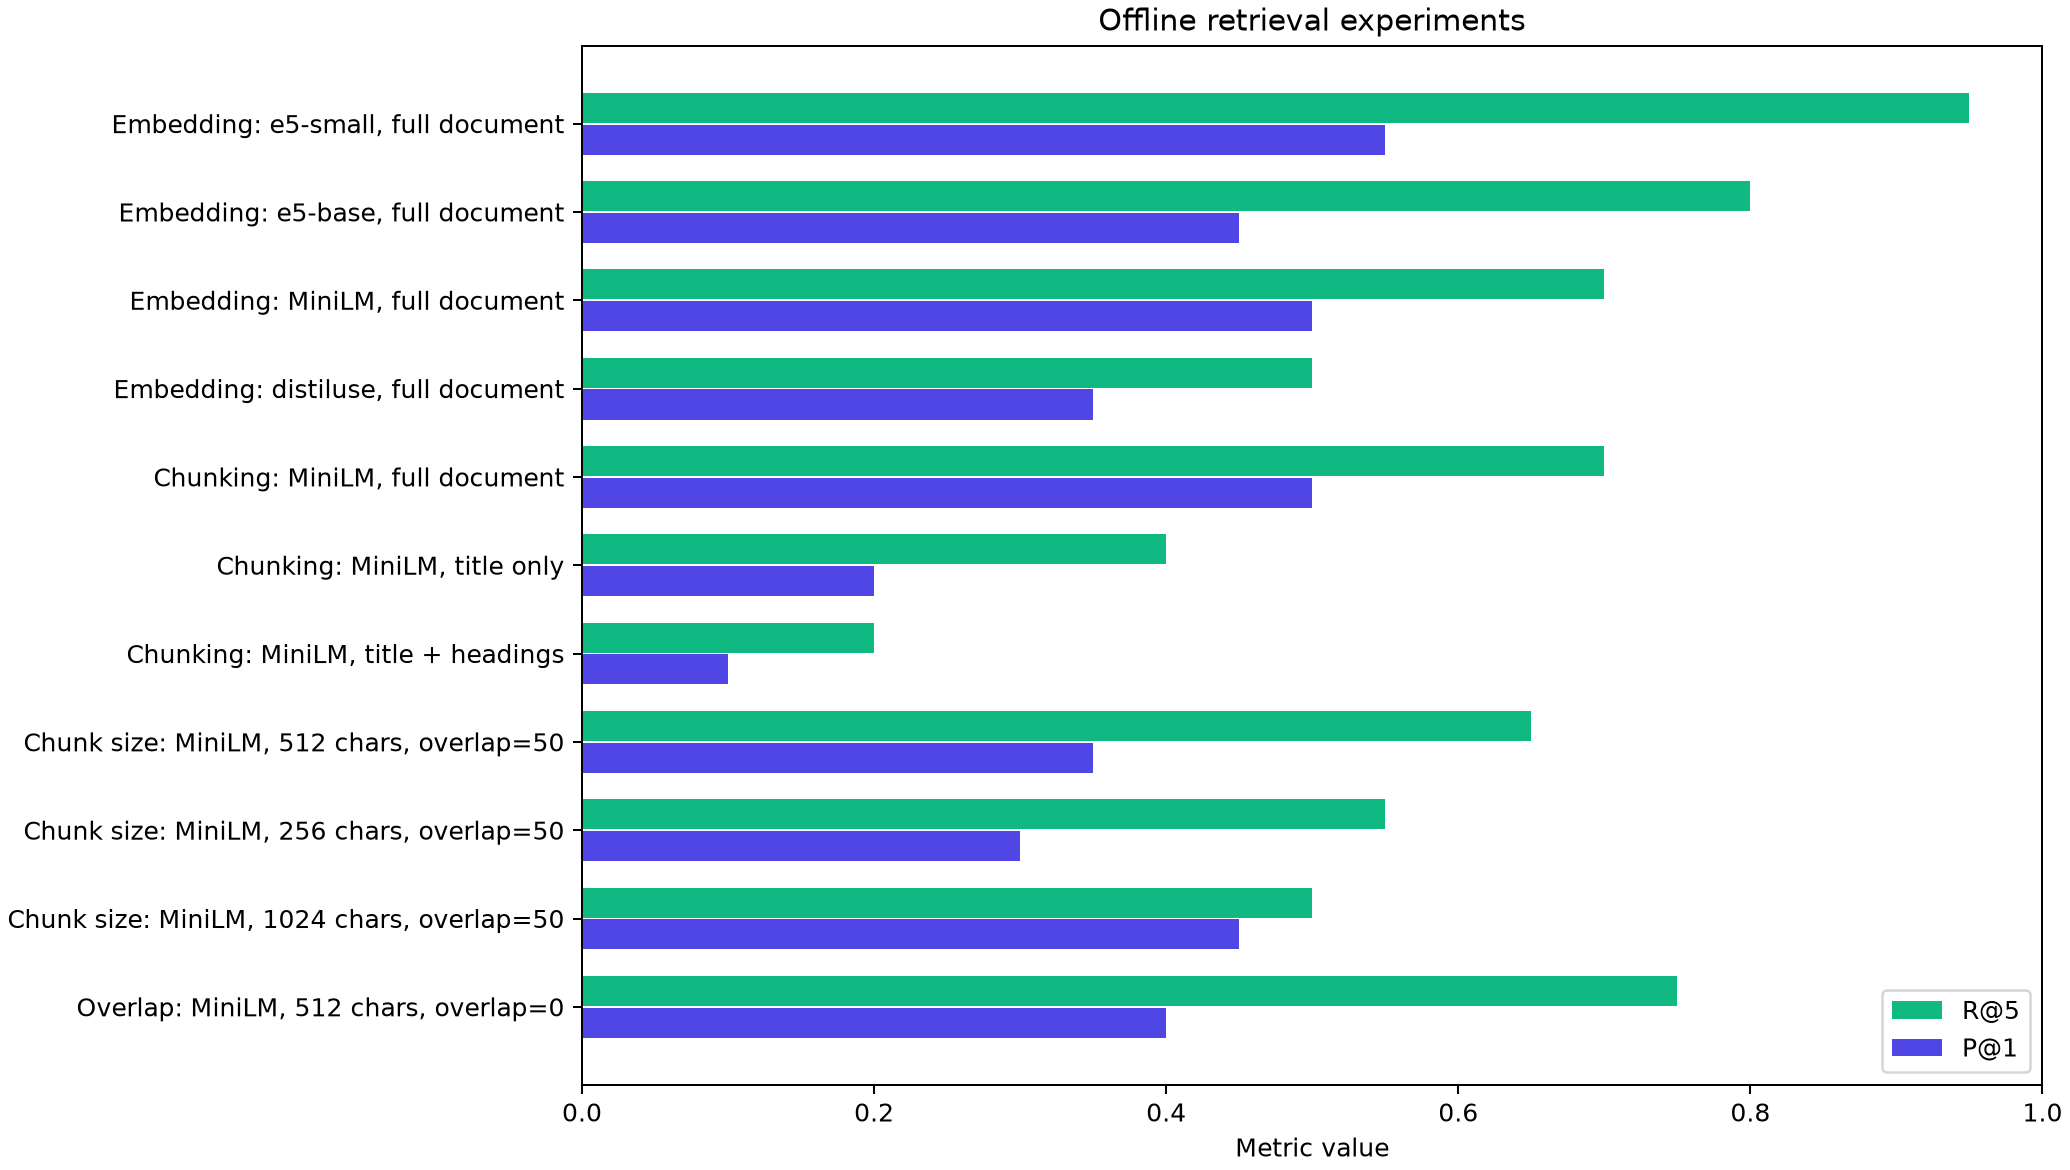
\includegraphics[width=\textwidth]{experiment_metrics.png}
    \end{column}
  \end{columns}

  \vspace{0.3em}
  \footnotesize
  Лучший offline retrieval среди зафиксированных MLflow-прогонов: \texttt{intfloat/multilingual-e5-small} на full-document представлении с $P@1 = 0.55$, $R@5 = 0.95$ и $MRR = 0.7125$.
\end{frame}

\begin{frame}{Интерпретация экспериментов}
  \small
  \begin{itemize}
    \item \textbf{Embedding comparison.} e5-small заметно лучше MiniLM по всем ключевым retrieval-метрикам; это означает, что модель лучше переносит пользовательские переформулировки и финансовую терминологию.
    \item \textbf{Chunking strategies.} Потеря полного текста резко ухудшает retrieval: одних заголовков и heading'ов недостаточно для точного семантического поиска, даже если структура статьи сохраняется.
    \item \textbf{Chunk size.} Среди завершенных прогонов лучший баланс дает размер 512 символов с overlap 50; слишком маленькие чанки теряют определение термина и дают более шумную выдачу.
    \item \textbf{Overlap.} В локальном MLflow полностью завершился только вариант overlap $= 0$; повторные прогоны остальных значений частично оборвались из-за внешнего доступа к моделям, поэтому по overlap пока делаем осторожные выводы.
    \item \textbf{Практический вывод.} Для сервиса разумна схема full-document dense retrieval + cross-encoder rerank; в production pipeline первым кандидатом на замену baseline является \texttt{multilingual-e5-small}.
  \end{itemize}
\end{frame}

\begin{frame}{Архитектура решения}
  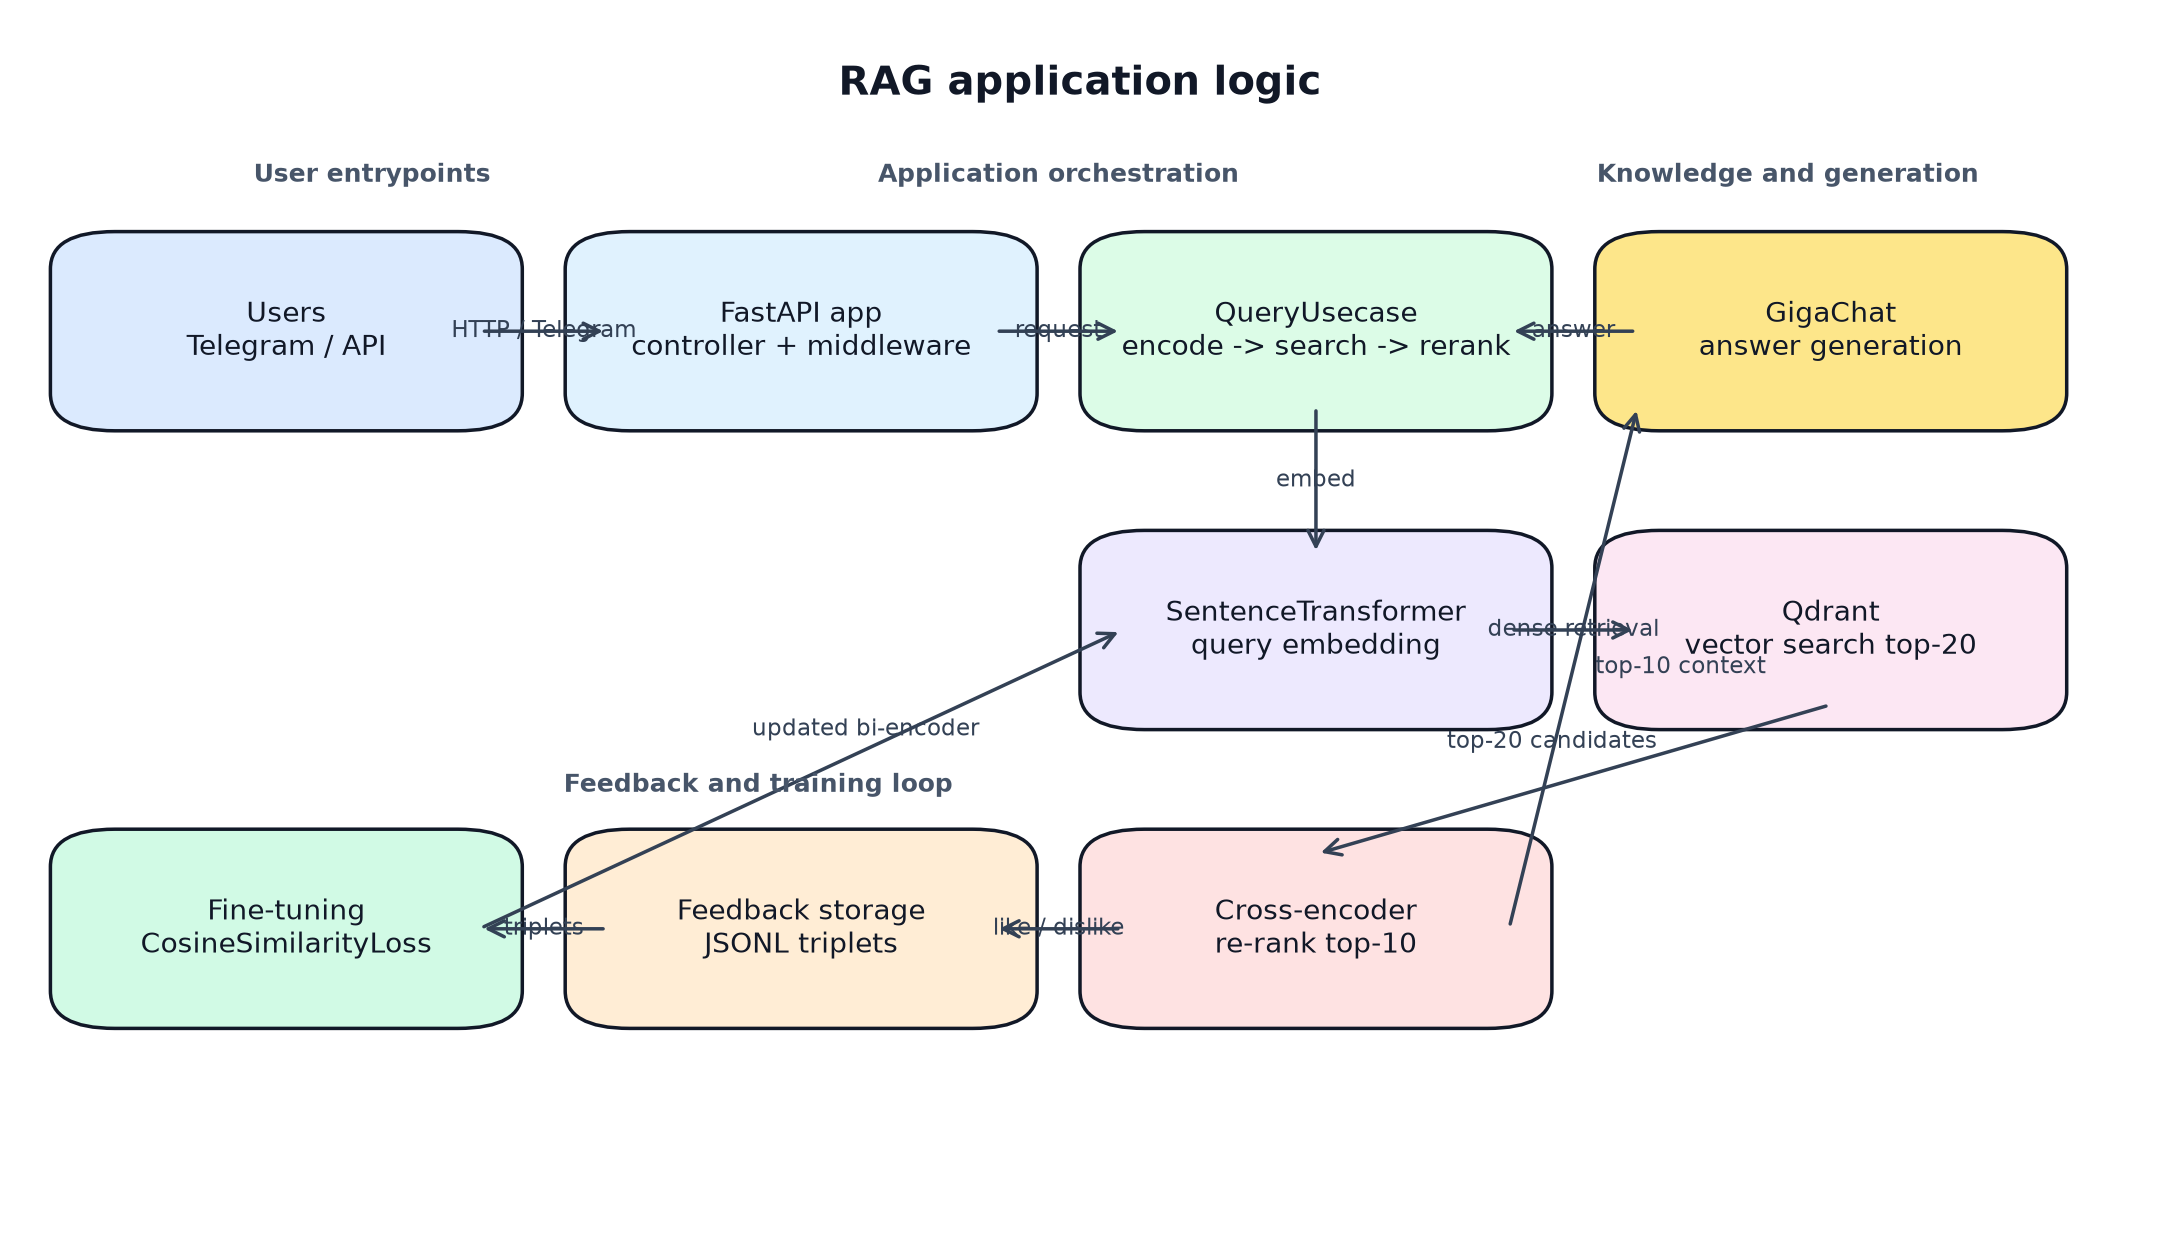
\includegraphics[width=\textwidth]{architecture_overview.png}
\end{frame}

\begin{frame}{Контейнеры и логика запуска}
  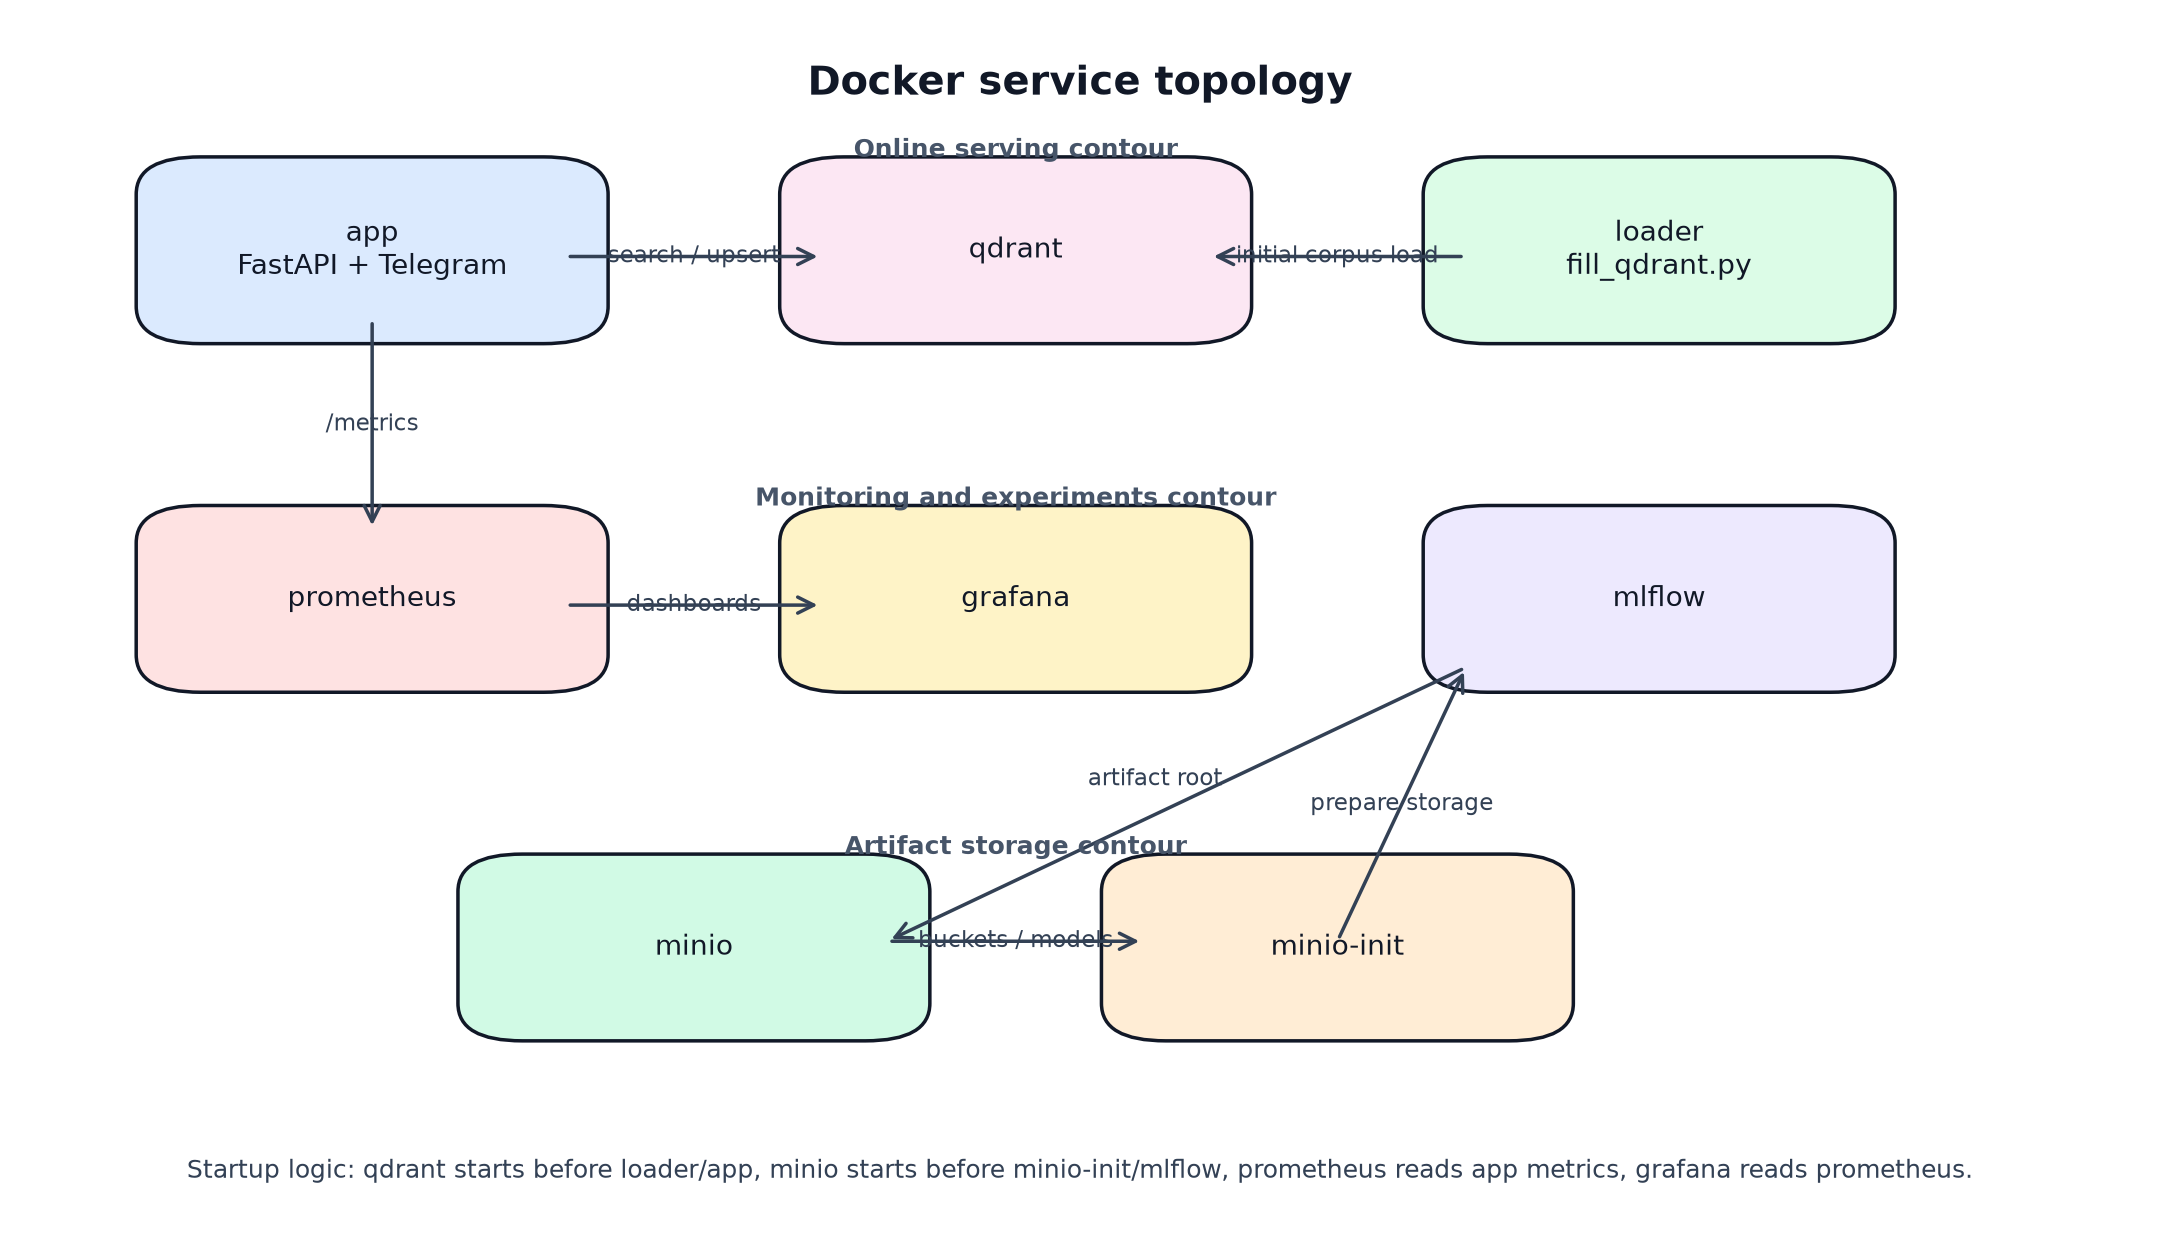
\includegraphics[width=\textwidth]{container_topology.png}
\end{frame}

\begin{frame}{Сервисная часть}
  \small
  \begin{itemize}
    \item Реализован FastAPI-сервис с endpoint'ами \texttt{/forward}, \texttt{/history}, \texttt{/stats}, \texttt{/health}, \texttt{/feedback}.
    \item Telegram-бот работает как внешний пользовательский интерфейс и лениво инициализирует RAG-компоненты при первом запросе.
    \item Qdrant хранит корпус в векторном виде; loader один раз наполняет коллекцию при старте инфраструктуры.
    \item MLflow и MinIO выделены в отдельную контурную часть для трекинга экспериментов и хранения артефактов; локальный sqlite backend позволяет воспроизводить результаты и без отдельного сервера.
    \item Для защиты можно вставить предзаписанное демо на 30--40 секунд как \texttt{service\_demo.gif} или \texttt{service\_demo.mp4}.
  \end{itemize}
  % \movie[width=0.72\textwidth,poster,showcontrols]{Demo}{presentation_assets/service_demo.mp4}
\end{frame}

\begin{frame}{Логирование и мониторинг}
  \small
  \textbf{Структурированные логи.}
  \begin{itemize}
    \item Каждый запрос проходит через middleware и получает \texttt{request\_id}.
    \item В JSON Lines логируются: \texttt{ts}, \texttt{level}, \texttt{logger}, \texttt{message}, \texttt{method}, \texttt{path}, \texttt{query}, \texttt{client\_ip}, \texttt{body}, \texttt{status\_code}, \texttt{duration\_ms}.
    \item Отдельно фиксируются этапы пайплайна: инициализация модели, embedding запроса, поиск в Qdrant, cross-encoder rerank, вызов GigaChat, отправка feedback.
    \item Для ошибок дополнительно пишутся \texttt{response\_body}, \texttt{exception} и контекст запроса, чтобы можно было разбирать сбои по конкретному сценарию пользователя.
  \end{itemize}

  \textbf{Prometheus / Grafana.}
  \begin{itemize}
    \item HTTP-метрики FastAPI собираются автоматически через instrumentator.
    \item Кастомные метрики RAG: \texttt{rag\_query\_duration\_seconds}, \texttt{rag\_embedding\_duration\_seconds}, \texttt{rag\_qdrant\_search\_duration\_seconds}, \texttt{rag\_rerank\_duration\_seconds}, \texttt{rag\_gigachat\_call\_duration\_seconds}, \texttt{rag\_gigachat\_errors\_total}, \texttt{rag\_feedback\_total}.
    \item Это позволяет отдельно видеть узкие места retrieval, rerank и внешнего LLM-вызова, а также различать проблемы качества ответа и проблемы времени отклика.
    \item На защиту можно добавить скрин Grafana с latency p95, числом ошибок внешнего LLM и динамикой feedback по дням.
  \end{itemize}
\end{frame}

\begin{frame}{Распределение ролей}
  \small
  \begin{itemize}
    \item \textbf{Охотин Даниил:} baseline RAG, BM25 + bi-encoder, адаптация retrieval под chunk-level корпус из \texttt{data/}, интеграция GigaChat, cross-encoder reranking, логика feedback loop, расчет retrieval-метрик.
    \item \textbf{Ващин Леонид:} сбор и очистка данных, подготовка Q\&A golden set, работа с источниками и подготовка дополнительных материалов корпуса.
    \item \textbf{Гусев Владислав:} FastAPI/Qdrant сервис, Docker-инфраструктура, Telegram UI для feedback, логирование, тесты, мониторинг и интеграционные исправления.
  \end{itemize}

  \vspace{0.3em}
  \footnotesize
  Формулировки восстановлены по README, changelog и истории commit'ов; перед финальной версией презентации их стоит синхронизировать с командой.
\end{frame}

\begin{frame}{Итоги}
  \small
  \begin{itemize}
    \item Собран и проанализирован корпус финансовых материалов, подготовлен golden set для offline-оценки retrieval.
    \item Построен и исследован RAG pipeline: baseline, embedding comparison, chunking, overlap, cross-encoder rerank.
    \item ML-эксперименты и презентационные артефакты адаптированы под реальный chunk-level формат папки \texttt{data/} с автоматическим восстановлением article/document-level представления.
    \item Лучший зафиксированный offline retrieval: \texttt{multilingual-e5-small}, $P@1 = 0.55$, $R@5 = 0.95$, $MRR = 0.7125$.
    \item Реализован production-ориентированный сервис: FastAPI + Qdrant + GigaChat + Telegram + feedback loop.
    \item Добавлены MLflow tracking, MinIO, Prometheus/Grafana и структурированное JSON-логирование.
  \end{itemize}

  \vspace{0.5em}
  GitHub: \href{https://github.com/bacchicsong/masters-project-rag}{github.com/bacchicsong/masters-project-rag}
\end{frame}

\end{document}
